\chapter{Six Questions With a Public CEO}

This chapter follows a School of Hard Knocks interview with Mark White, presented here as a source-conscious companion text curated by LazyingArt LLC through Video2Book. There is no blackboard calculation in this source. The mathematical structure we use is therefore not imported physics, but disciplined bookkeeping: we separate anecdote, claim, and mechanism, and we write the mechanisms as compact maps so that the commercial judgment can be inspected rather than merely admired.

\section{The Opening Frame: A Public CEO and a Practical Question}

James Newman begins by giving us the reason to listen. A few weeks earlier, the show had interviewed Mark White of Nexalyn Technologies, a public-company CEO who describes his business as helping people get off psychiatric medication and using frequencies to restore mental health. The host then says White invited them to his headquarters in Houston, Texas, to give young entrepreneurs more practical game.

The setup matters because it creates a tension. We are not first shown a balance sheet, a stock chart, or a theory of entrepreneurship. We are given a person who has reached a public-company role and then asked to trace backward: what concrete behaviors, judgments, and scars made that possible?

For this chapter, the useful object is a mechanism:
\begin{equation}
\text{business lesson}
=
\text{anecdote}
+
\text{claim}
+
\text{repeatable mechanism}.
\end{equation}
The anecdote keeps the source honest. The claim tells us what the speaker thinks the anecdote means. The mechanism is the part a reader can test in another setting.

\section{First Money: Valet Access Becomes a Car-Detailing Offer}

The first direct question is simple: what was the first business? White answers just as simply: car detailing. Then he reconstructs the setting. He was a valet parker at a Houston hotel during the late-1970s oil boom, at the new Galleria, when many nice restaurants were still inside hotels. Customers would drive in, hand over the car, and disappear into dinner.

That gave him three assets before he had a company: access to the car, a window of idle time, and a visible way to improve the customer's property. Armor All was new. Cleaning a wheel and treating a tire could make the car look newly refreshed. White and the doorman turned that observation into an offer: while the customer was at dinner, they could wash and detail the car. The price he names is \(\$20\).

\subsection{Question \& Answer}

\paragraph{Question.} What was the first real money-making mechanism?

\paragraph{Answer.} It was not a grand plan. It was controlled access plus a small visible transformation. The customer had already trusted the valet with the car; dinner created time; Armor All created a clear before-and-after result; and the \(\$20\) offer made the experiment small enough to accept.

A compact reconstruction is:
\begin{equation}
\text{Opportunity}
\approx
\text{access}
+
\text{idle time}
+
\text{visible improvement}
+
\text{small offer}.
\end{equation}

The first business did not require a storefront. White says he parked cars at night and, in the mornings, picked up Lincoln Mark Fives and Cadillac Eldorados from customers' offices, took them to his house, cleaned the wheels with a toothbrush, and Armor Alled the tires. In the chapter's broader book structure, this belongs under the question: what was the first real money-making mechanism?

\begin{figure}
\centering
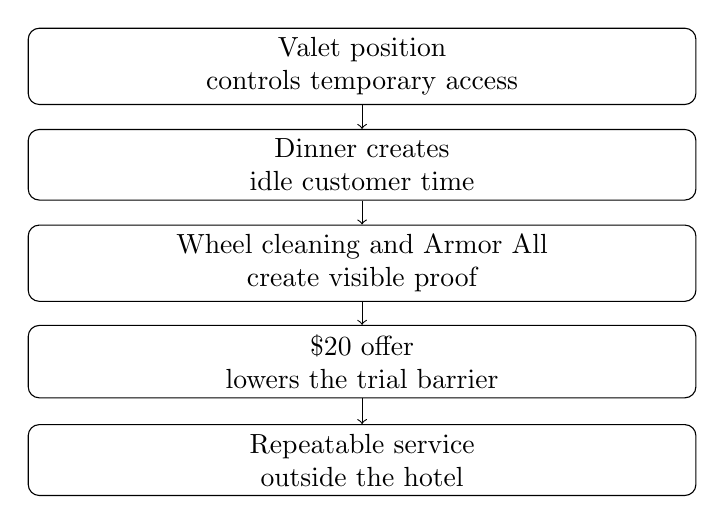
\begin{tikzpicture}
\node[draw, rounded corners, align=center, text width=.68\linewidth] (a) at (0,0) {Valet position\\controls temporary access};
\node[draw, rounded corners, align=center, text width=.68\linewidth] (b) at (0,-1.25) {Dinner creates\\idle customer time};
\node[draw, rounded corners, align=center, text width=.68\linewidth] (c) at (0,-2.50) {Wheel cleaning and Armor All\\create visible proof};
\node[draw, rounded corners, align=center, text width=.68\linewidth] (d) at (0,-3.75) {\(\$20\) offer\\lowers the trial barrier};
\node[draw, rounded corners, align=center, text width=.68\linewidth] (e) at (0,-5.00) {Repeatable service\\outside the hotel};
\draw[->] (a) -- (b);
\draw[->] (b) -- (c);
\draw[->] (c) -- (d);
\draw[->] (d) -- (e);
\end{tikzpicture}
\caption{A transcript-grounded reconstruction of the car-detailing mechanism.}
\end{figure}

\section{Sales Without the Hard Close}

The host next asks about sales. White acknowledges the old sales-school world, naming Zig Ziglar and Tony Robbins, but he does not frame his own method as closing tricks. His answer is communication. He says he has energy, confidence, and has learned how to communicate. The important distinction is that selling, for him, is not mainly asking for the deal. It is communicating with people from a place of belief in the product or service.

That belief creates what he calls a natural sales moment. If he is talking about Nexalyn technology, mind care, brain training, or brain stimulation, he expects the listener to see that he loves what he does. Then human curiosity does part of the work: the listener wants to know what is driving that confidence.

\subsection{Question \& Answer}

\paragraph{Question.} What is the secret to sales in this interview?

\paragraph{Answer.} The secret is not pressure. It is a loop of inquiry, listening, adjustment, and respect. White says that when he walks into a room, one of the first things he asks himself is why they would say no. Then he asks questions, listens to the response, and tailors the message.

We can write the sales loop as:
\begin{equation}
\text{Ask}
\longrightarrow
\text{Listen}
\longrightarrow
\text{Tailor}
\longrightarrow
\text{Respect}
\longrightarrow
\text{Engage}.
\end{equation}

The respect term is not decorative. White says he does not want to tell people something they do not want to know, nor tell them something they already know better than he does. In a room with medical professionals, his first move is humility: he is not there to pretend he knows healthcare better than they do. He is there, as he frames it, to offer a vision of what he thinks could be a better healthcare system.

\section{Fewer Words, Careful Money, and Humility}

The next question asks for the best advice he ever received from a mentor. White's first answer is compact and almost corrective: talk too much; slow down; say what you are going to say in fewer words, because the people listening do not know it as well as you know it.

Then he moves to money. In entrepreneurial life, he says, personal and professional finances come together. A company has a big week, a few thousand dollars come in, and suddenly the founder is buying a suit at Saks Fifth Avenue or a \(\$200\) bottle of wine. The lesson is not that one purchase ruins a company. The lesson is that a founder's personal impulse can leak out of the same capital pool that the business needs to survive.

\begin{equation}
\text{business income}
+
\text{personal spending impulse}
\longrightarrow
\text{capital leakage}.
\end{equation}

\subsection{Question \& Answer}

\paragraph{Question.} How can confidence and humility coexist?

\paragraph{Answer.} White's answer is that confidence is not the same as pretending. He says he is confident and aggressive, but tries to stay aware of what he does not know. Humility becomes an operating constraint: do not over-explain, do not overspend, do not outrank the expert in the room, and do not confuse firsthand knowledge with wisdom.

He gives the distinction in plain language:
\begin{align}
\text{knowledge} &\approx \text{firsthand experience},\\
\text{wisdom} &\approx \text{listening to those with knowledge}.
\end{align}
That distinction becomes a hinge. The interview is no longer only about making money. It is about how experience is turned into judgment.

\section{Trauma, the Brain, and an Attributed Two-System Model}

The host then pivots sharply. He introduces Kanye West as a public example of someone who had a close relationship with his mother, then seemed to move through controversy, mental-health concern, medication, and visible weight gain. The question is not about business directly. It is about trauma: how can the loss of a relationship affect the brain?

White begins by broadening the word trauma. In his framing, trauma is not only a major injury. It can be anything abnormal in day-to-day life experience. He names three main forms:
\begin{equation}
\text{Trauma}
=
\{\text{toxic},\ \text{physical},\ \text{emotional}\}.
\end{equation}
Toxic trauma includes addiction, alcohol, drugs, food sensitivity, and poisons. Physical trauma includes football injuries, falling off a bicycle, head injury, traumatic brain injury, and war injuries. Emotional trauma includes loss of a loved one and betrayal by a loved one.

\subsection{Question \& Answer}

\paragraph{Question.} How does relationship trauma affect the brain, according to Mark White?

\paragraph{Answer.} White's claim is that the brain has two systems, an electrical system and a chemical system, and that trauma can disturb one or both. He describes these systems as doing a kind of dance. Their job, in his language, is to help a person handle life on life's terms.

The claim can be recorded cautiously as:
\begin{equation}
\text{brain system}
=
\text{chemical system}
+
\text{electrical system}.
\end{equation}
He then links trauma to the fight-or-flight response. In the moment, the brain protects the person. After the event, however, the system may not return cleanly to balance. That is where he brings in PTSD, emphasizing that it is not only military. In his examples, PTSD can follow a bad marriage, a bad employer, or the loss of a loved one.

White's attributed model of manifestation is:
\begin{equation}
\text{trauma response}
\longrightarrow
\{\text{chemical imbalance},\ \text{EEG/frequency disturbance}\}.
\end{equation}
He names dopamine, serotonin, and acetylcholine as chemical examples, and EEG or frequencies as the electrical side. The chapter should keep this language attached to White's view. It should not convert the interview into independent medical proof.

\subsection{Treatment Claims and Caution}

White argues that, with fairness to doctors and psychiatrists, some psychiatric treatment can become a guessing game: a patient says he feels depressed or has lost desire in life, and a medication such as Prozac is tried. He characterizes this as chemically altering a chemically altered brain and says it may work some of the time but not all the time.

His preferred starting point is also stated as a claim: treatment should begin, in his humble opinion, with non-invasive technologies, nutrition, talk therapy or talking to a friend, and the foundations of life. He also says he is a man of faith and believes in belonging to a spiritual community.

The practical pattern he emphasizes is gradualism. You do not get into a condition overnight, and you do not get out of it overnight. His analogy is weight gain: a person does not gain a hundred pounds overnight and should not expect to lose a hundred pounds overnight.

\section{Failure as the Greatest Accomplishment}

The host returns to entrepreneurship: White has started companies and brought a company public, so what is his greatest accomplishment? The expected answer might be the public company. White gives the reversal: getting up, brushing himself off, licking his wounds, and going back in for another round.

He says the worst thing after never having money is having a lot of money, losing it, and then not having any money. The central scene is brutal: watching his life's work get loaded into trucks and taken down the road. He names a bankruptcy attorney, rendered in the transcript as Nelson Hemsley, who told him he could either pay the attorney to go to court and clean up the mess, or he could come to every meeting, go to the courthouse, and face the people he owed money to.

\subsection{Question \& Answer}

\paragraph{Question.} Why is failure, rather than going public, named as the greatest accomplishment?

\paragraph{Answer.} Because the failure forced accountability. White says his greatest accomplishment was having the strength and nerve to go into a room of people who hated him because he had failed, owed them money, and they lost money. He does not present this as a clean inspirational slogan. He presents it as humiliation, restitution, and rebuilding.

The mechanism is:
\begin{equation}
\text{failure}
+
\text{creditor-facing accountability}
+
\text{humility}
\longrightarrow
\text{practical wisdom}.
\end{equation}

The ordered lesson is worth making explicit:
\begin{enumerate}
\item A business failure creates obligations to real people.
\item Avoiding those people may preserve comfort, but it loses the lesson.
\item Facing them converts failure into accountability.
\item Giving assets back and watching them be divided and sold imposes humility.
\item On the other side, White says he became a new man.
\end{enumerate}

That last phrase includes more than business. He says he gained a new level of respect for his fellow man, remarried his wife, put his family back together, and learned humility. The transcript repeats the word humility, and the repetition is justified. It is one of the controlling ideas of the whole interview.

\section{Structure as Self-Improvement}

The closing turn is practical. The host asks whether White reads. White says he is not a reader; he is a skimmer. Then comes the self-improvement question: what should the average modern man do if he is out of shape, addicted to Netflix and dopamine, and wants to get serious?

White answers with one word: structure.

He tells a story about a man named Haas. Haas told him to set an alarm for 8 a.m., get out of bed, make the bed, shower, be ready at 9 a.m., eat lunch at noon, eat dinner at six, prepare for bed at night, and get in bed. White's response was: that's it? Haas's answer was the point: you need to be successful at something.

This is an update rule for self-trust:
\begin{align}
S_{n+1} &= S_n + \delta, \qquad \delta > 0
        \quad \text{if today's promise is kept},\\
S_{n+1} &= S_n - \epsilon, \qquad \epsilon > 0
        \quad \text{if the promise is abandoned}.
\end{align}
Here \(S_n\) is not a clinical variable. It is just a bookkeeping symbol for self-trust after \(n\) days. The rule captures White's point: the task is small, but the evidence matters. At the end of the day, the person can sit quietly and say, I did what I said I would do.

\subsection{A Worked Example}

Suppose the only promise is this: wake at 8 a.m., make the bed, and be on time to work. Let the starting self-trust be \(S_0=0\). If a kept promise adds \(1\) unit and a broken promise subtracts \(2\), then five days with the pattern
\[
\text{kept},\ \text{kept},\ \text{broken},\ \text{kept},\ \text{kept}
\]
gives
\begin{align}
S_1 &= 0+1=1,\\
S_2 &= 1+1=2,\\
S_3 &= 2-2=0,\\
S_4 &= 0+1=1,\\
S_5 &= 1+1=2.
\end{align}
The numbers are invented, but the direction is White's mechanism. A person does not rebuild by declaring a total transformation. He rebuilds by choosing a small promise, keeping it, noticing that it was kept, and repeating.

White contrasts this with the New Year's resolution pattern. A person tries to stop A, B, C, D and start E, F, G, H all at once. He gets through A and B, fails, feels shame and disappointment, turns on Netflix, gets chips, and starts over. The correction is not grandiosity. It is a smaller unit of success.

\begin{figure}
\centering
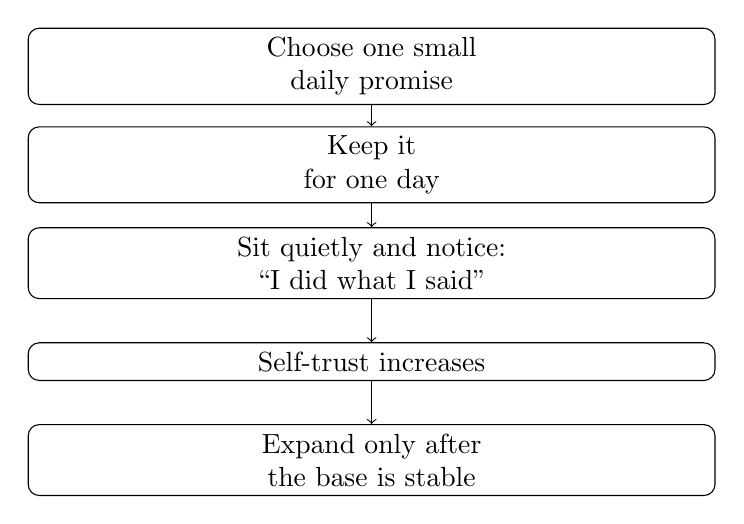
\begin{tikzpicture}
\node[draw, rounded corners, align=center, text width=.70\linewidth] (a) at (0,0) {Choose one small\\daily promise};
\node[draw, rounded corners, align=center, text width=.70\linewidth] (b) at (0,-1.25) {Keep it\\for one day};
\node[draw, rounded corners, align=center, text width=.70\linewidth] (c) at (0,-2.50) {Sit quietly and notice:\\``I did what I said''};
\node[draw, rounded corners, align=center, text width=.70\linewidth] (d) at (0,-3.75) {Self-trust increases};
\node[draw, rounded corners, align=center, text width=.70\linewidth] (e) at (0,-5.00) {Expand only after\\the base is stable};
\draw[->] (a) -- (b);
\draw[->] (b) -- (c);
\draw[->] (c) -- (d);
\draw[->] (d) -- (e);
\end{tikzpicture}
\caption{The self-improvement mechanism reconstructed from the Haas routine.}
\end{figure}

\section{Summary}

The interview begins with the authority of a public CEO, but its durable lessons come from smaller scenes: a valet spotting a \(\$20\) detailing opportunity, a salesman asking why the customer might say no, a founder warned not to let a good week turn into capital leakage, a health entrepreneur describing trauma through his own attributed two-system model, a failed businessman facing creditors, and a struggling person rebuilding from one kept promise.

The common structure is not luck. It is attention to mechanisms. Access can become opportunity. Communication can replace pressure. Humility can protect judgment. Failure can become education when it is faced directly. Structure can rebuild self-trust when it is small enough to keep.